\documentclass{standalone}
\usepackage{tikz}
\usetikzlibrary{patterns, positioning}
\usepackage[sfdefault]{ClearSans} %% option 'sfdefault' activates Clear Sans as the default text font
\usepackage[T1]{fontenc}

\begin{document}
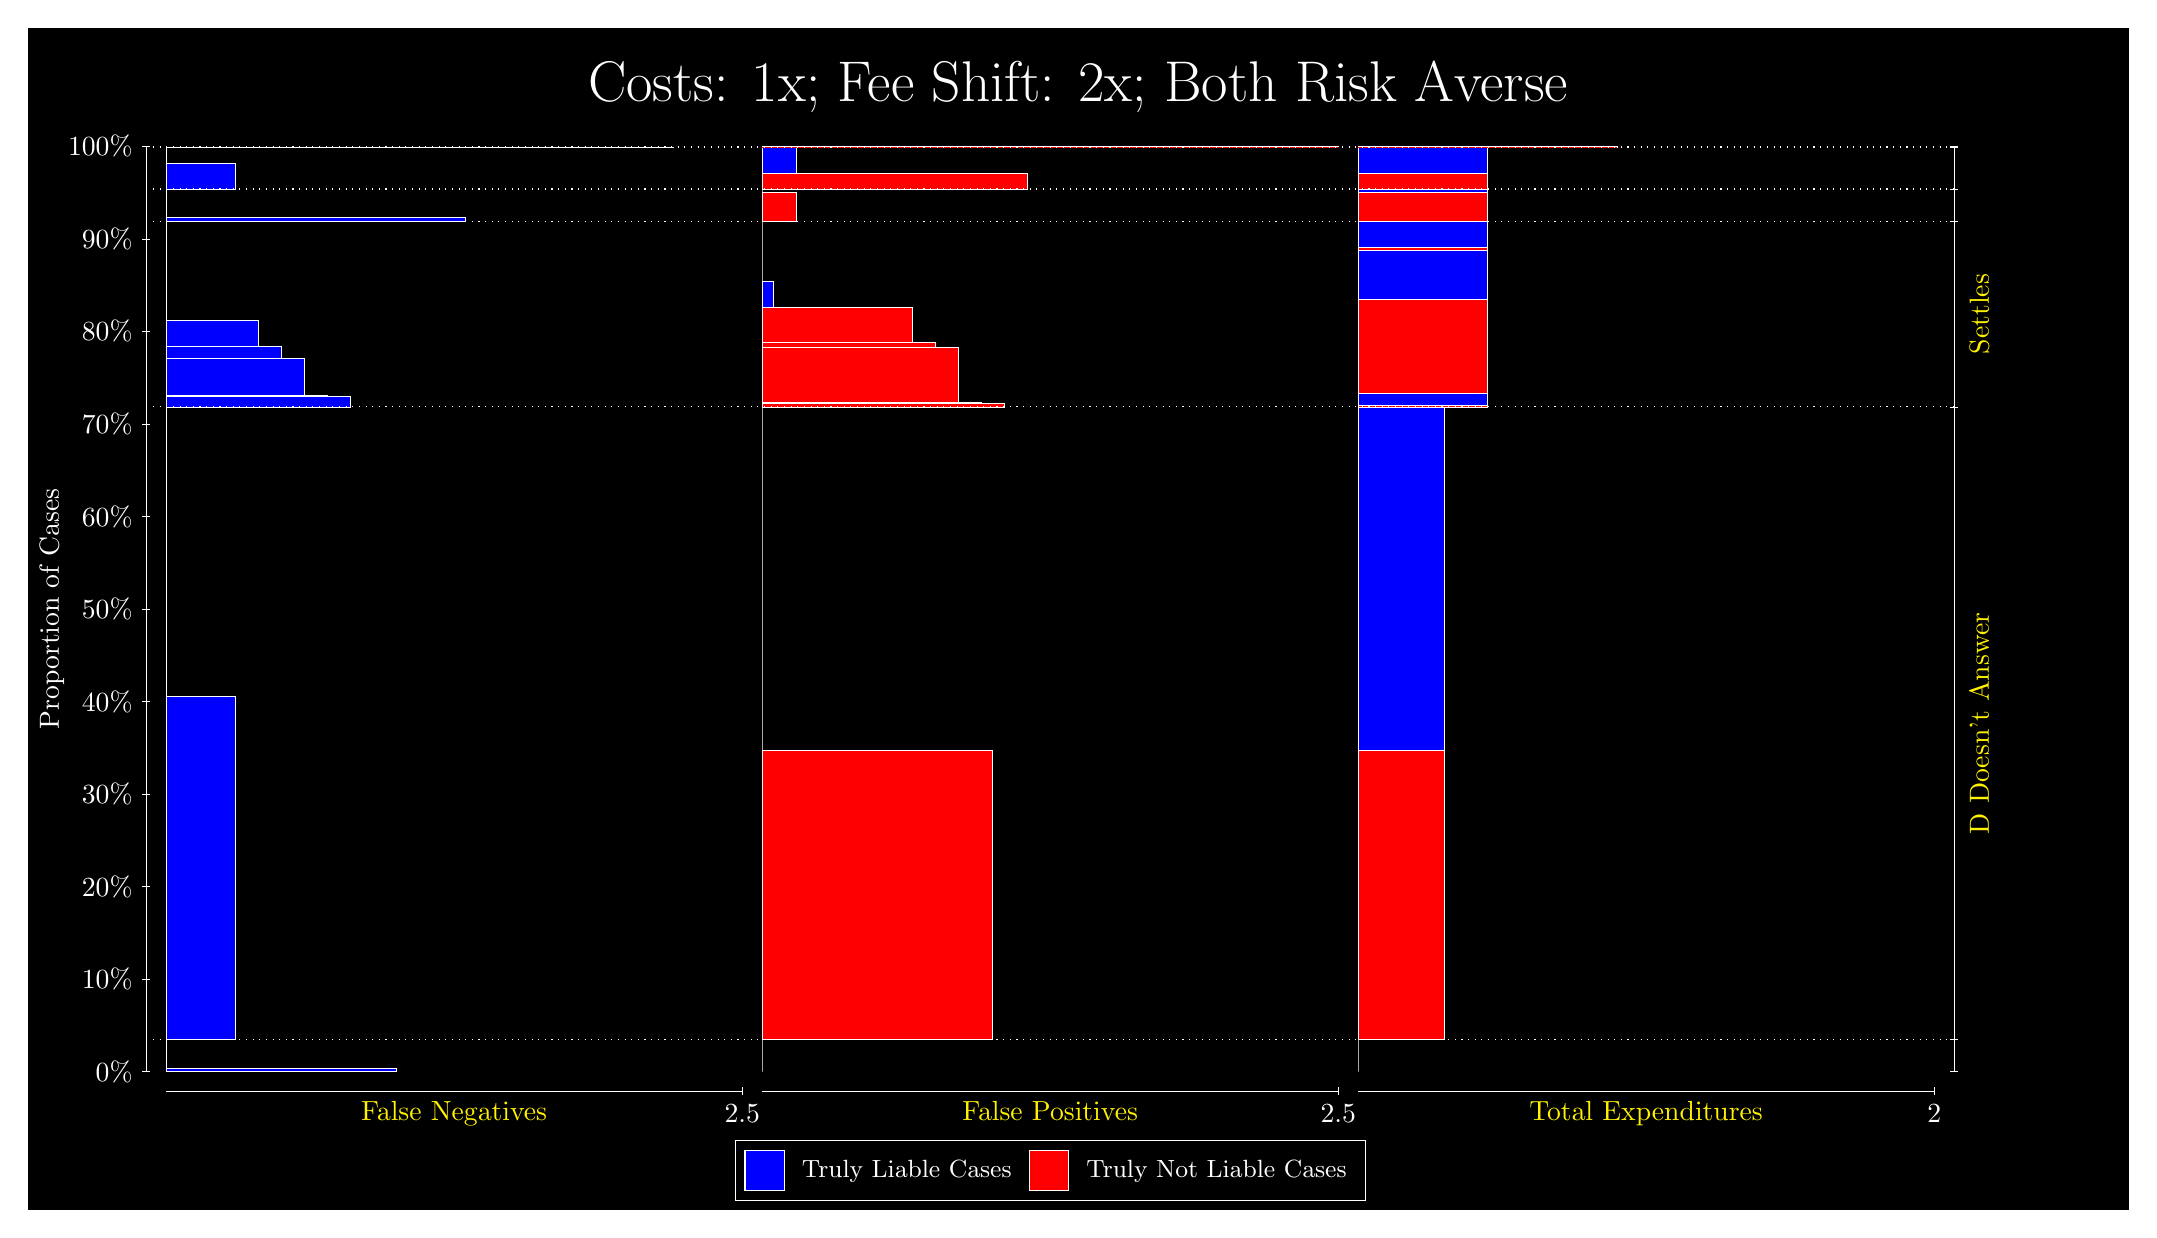
\begin{tikzpicture}
\draw[fill=black] (0,0) rectangle (26.667,15);
\draw[text=white] (0,13.5) rectangle (26.667,15) node[midway] {\huge Costs: 1x; Fee Shift: 2x; Both Risk Averse};
\draw[white, very thin] (1.5,1.75) -- (1.5,13.5);
\node[rotate=90, text=white, anchor=center] at (0.3, 7.625) {Proportion of Cases};
\draw[white, very thin] (1.45,1.75) -- (1.55,1.75);
\node[text=white, anchor=east] at (1.45, 1.75) {0\%};
\draw[white, very thin] (1.45,2.925) -- (1.55,2.925);
\node[text=white, anchor=east] at (1.45, 2.925) {10\%};
\draw[white, very thin] (1.45,4.1) -- (1.55,4.1);
\node[text=white, anchor=east] at (1.45, 4.1) {20\%};
\draw[white, very thin] (1.45,5.275) -- (1.55,5.275);
\node[text=white, anchor=east] at (1.45, 5.275) {30\%};
\draw[white, very thin] (1.45,6.45) -- (1.55,6.45);
\node[text=white, anchor=east] at (1.45, 6.45) {40\%};
\draw[white, very thin] (1.45,7.625) -- (1.55,7.625);
\node[text=white, anchor=east] at (1.45, 7.625) {50\%};
\draw[white, very thin] (1.45,8.8) -- (1.55,8.8);
\node[text=white, anchor=east] at (1.45, 8.8) {60\%};
\draw[white, very thin] (1.45,9.975) -- (1.55,9.975);
\node[text=white, anchor=east] at (1.45, 9.975) {70\%};
\draw[white, very thin] (1.45,11.15) -- (1.55,11.15);
\node[text=white, anchor=east] at (1.45, 11.15) {80\%};
\draw[white, very thin] (1.45,12.325) -- (1.55,12.325);
\node[text=white, anchor=east] at (1.45, 12.325) {90\%};
\draw[white, very thin] (1.45,13.5) -- (1.55,13.5);
\node[text=white, anchor=east] at (1.45, 13.5) {100\%};

\draw[white, very thin] (24.457,1.75) -- (24.457,13.5);
\draw[white, very thin] (24.407,1.75) -- (24.507,1.75);
\node[anchor=west] at (24.407, 1.75) {};
\draw[white, very thin] (24.407,2.1553) -- (24.507,2.1553);
\node[anchor=west] at (24.407, 2.1553) {};
\draw[white, very thin] (24.407,10.191) -- (24.507,10.191);
\node[anchor=west] at (24.407, 10.191) {};
\draw[white, very thin] (24.407,12.549) -- (24.507,12.549);
\node[anchor=west] at (24.407, 12.549) {};
\draw[white, very thin] (24.407,12.958) -- (24.507,12.958);
\node[anchor=west] at (24.407, 12.958) {};
\draw[white, very thin] (24.407,13.484) -- (24.507,13.484);
\node[anchor=west] at (24.407, 13.484) {};
\draw[white, very thin] (24.407,13.495) -- (24.507,13.495);
\node[anchor=west] at (24.407, 13.495) {};
\draw[white, very thin] (24.407,13.5) -- (24.507,13.5);
\node[anchor=west] at (24.407, 13.5) {};

\draw[white, very thin, fill=blue] (1.75,1.75) rectangle (4.6775,1.7926);
\draw[white, very thin, fill=red] (1.75,1.7926) rectangle (1.75,2.1553);
\draw[white, very thin, fill=blue] (1.75,2.1553) rectangle (2.6283,6.5156);
\draw[white, very thin, fill=red] (1.75,6.5156) rectangle (1.75,10.191);
\draw[white, very thin, fill=blue] (1.75,10.191) rectangle (4.092,10.328);
\draw[white, very thin, fill=blue] (1.75,10.328) rectangle (3.7993,10.334);
\draw[white, very thin, fill=blue] (1.75,10.334) rectangle (3.5065,10.812);
\draw[white, very thin, fill=blue] (1.75,10.812) rectangle (3.2138,10.96);
\draw[white, very thin, fill=blue] (1.75,10.96) rectangle (2.921,11.289);
\draw[white, very thin, fill=red] (1.75,11.289) rectangle (1.75,12.549);
\draw[white, very thin, fill=blue] (1.75,12.549) rectangle (5.5558,12.595);
\draw[white, very thin, fill=red] (1.75,12.595) rectangle (1.75,12.958);
\draw[white, very thin, fill=blue] (1.75,12.958) rectangle (2.6283,13.281);
\draw[white, very thin, fill=red] (1.75,13.281) rectangle (1.75,13.484);
\draw[white, very thin, fill=blue] (1.75,13.484) rectangle (8.1906,13.486);
\draw[white, very thin, fill=red] (1.75,13.486) rectangle (1.75,13.495);
\draw[white, very thin, fill=red] (1.75,13.495) rectangle (1.75,13.497);
\draw[white, very thin, fill=blue] (1.75,13.497) rectangle (1.75,13.5);
\draw[white, very thin, fill=red] (9.3189,1.75) rectangle (9.3189,2.1126);
\draw[white, very thin, fill=blue] (9.3189,2.1126) rectangle (9.3189,2.1553);
\draw[white, very thin, fill=red] (9.3189,2.1553) rectangle (12.246,5.8305);
\draw[white, very thin, fill=blue] (9.3189,5.8305) rectangle (9.3189,10.191);
\draw[white, very thin, fill=red] (9.3189,10.191) rectangle (12.393,10.231);
\draw[white, very thin, fill=red] (9.3189,10.231) rectangle (12.1,10.254);
\draw[white, very thin, fill=red] (9.3189,10.254) rectangle (11.807,10.946);
\draw[white, very thin, fill=red] (9.3189,10.946) rectangle (11.515,11.009);
\draw[white, very thin, fill=red] (9.3189,11.009) rectangle (11.222,11.452);
\draw[white, very thin, fill=blue] (9.3189,11.452) rectangle (9.4652,11.781);
\draw[white, very thin, fill=blue] (9.3189,11.781) rectangle (9.3189,12.549);
\draw[white, very thin, fill=red] (9.3189,12.549) rectangle (9.758,12.913);
\draw[white, very thin, fill=blue] (9.3189,12.913) rectangle (9.3189,12.958);
\draw[white, very thin, fill=red] (9.3189,12.958) rectangle (12.686,13.16);
\draw[white, very thin, fill=blue] (9.3189,13.16) rectangle (9.758,13.484);
\draw[white, very thin, fill=red] (9.3189,13.484) rectangle (9.3189,13.492);
\draw[white, very thin, fill=blue] (9.3189,13.492) rectangle (9.3189,13.495);
\draw[white, very thin, fill=red] (9.3189,13.495) rectangle (16.638,13.497);
\draw[white, very thin, fill=blue] (9.3189,13.497) rectangle (13.71,13.5);
\draw[white, very thin, fill=red] (16.888,1.75) rectangle (16.888,2.1126);
\draw[white, very thin, fill=blue] (16.888,2.1126) rectangle (16.888,2.1553);
\draw[white, very thin, fill=red] (16.888,2.1553) rectangle (17.986,5.8305);
\draw[white, very thin, fill=blue] (16.888,5.8305) rectangle (17.986,10.191);
\draw[white, very thin, fill=red] (16.888,10.191) rectangle (18.534,10.214);
\draw[white, very thin, fill=blue] (16.888,10.214) rectangle (18.534,10.362);
\draw[white, very thin, fill=red] (16.888,10.362) rectangle (18.534,11.56);
\draw[white, very thin, fill=blue] (16.888,11.56) rectangle (18.534,12.18);
\draw[white, very thin, fill=red] (16.888,12.18) rectangle (18.534,12.221);
\draw[white, very thin, fill=blue] (16.888,12.221) rectangle (18.534,12.549);
\draw[white, very thin, fill=red] (16.888,12.549) rectangle (18.534,12.913);
\draw[white, very thin, fill=blue] (16.888,12.913) rectangle (18.534,12.958);
\draw[white, very thin, fill=red] (16.888,12.958) rectangle (18.534,13.16);
\draw[white, very thin, fill=blue] (16.888,13.16) rectangle (18.534,13.484);
\draw[white, very thin, fill=red] (16.888,13.484) rectangle (20.181,13.492);
\draw[white, very thin, fill=blue] (16.888,13.492) rectangle (20.181,13.495);
\draw[white, very thin, fill=red] (16.888,13.495) rectangle (20.181,13.497);
\draw[white, very thin, fill=blue] (16.888,13.497) rectangle (20.181,13.5);
\draw[white, dotted] (1.5,2.1553) -- (24.457,2.1553);
\draw[white, dotted] (1.5,10.191) -- (24.457,10.191);
\draw[white, dotted] (1.5,12.549) -- (24.457,12.549);
\draw[white, dotted] (1.5,12.958) -- (24.457,12.958);
\draw[white, dotted] (1.5,13.484) -- (24.457,13.484);
\draw[white, dotted] (1.5,13.495) -- (24.457,13.495);
\draw[white, very thin] (1.75,1.5) -- (9.0689,1.5);
\node[text=yellow, anchor=north] at (5.4094, 1.5) {False Negatives};
\draw[white, very thin] (9.0689,1.45) -- (9.0689,1.55);
\node[text=white, anchor=north] at (9.0689, 1.45) {2.5};

\draw[white, very thin] (9.3189,1.5) -- (16.638,1.5);
\node[text=yellow, anchor=north] at (12.978, 1.5) {False Positives};
\draw[white, very thin] (16.638,1.45) -- (16.638,1.55);
\node[text=white, anchor=north] at (16.638, 1.45) {2.5};

\draw[white, very thin] (16.888,1.5) -- (24.207,1.5);
\node[text=yellow, anchor=north] at (20.547, 1.5) {Total Expenditures};
\draw[white, very thin] (24.207,1.45) -- (24.207,1.55);
\node[text=white, anchor=north] at (24.207, 1.45) {2};


\node[text=yellow, centered, rotate=90] at (24.777, 6.1731) {D Doesn't Answer};
\node[text=yellow, centered, rotate=90] at (24.777, 11.37) {Settles};





\draw (12.978300999999998,1.5) node[draw=none] (baseCoordinate) {};
\begin{scope}[align=center]
        \matrix[scale=0.5, draw=white, below=0.5cm of baseCoordinate, nodes={draw}, column sep=0.1cm]{
            \node[rectangle, draw, minimum width=0.5cm, minimum height=0.5cm, fill=blue] {}; &
            \node[draw=none, font=\small, text=white] (B) {Truly Liable Cases}; &
            \node[rectangle, draw, minimum width=0.5cm, minimum height=0.5cm, fill=red] {}; &
            \node[draw=none, font=\small, text=white] (B) {Truly Not Liable Cases}; \\
            };
\end{scope}

\end{tikzpicture}
\end{document}